\documentclass[16pt,answers]{exam}
\author{Nima Poshtiban}
\title{Digital Electronics}
\usepackage{datetime}
\newdate{date}{26}{10}{2025}
\newdate{due}{1}{11}{2025}
\date{\displaydate{date}}
\usepackage[utf8]{inputenc}
\usepackage{amsmath}
\usepackage{enumitem}
\usepackage{graphicx}
\usepackage[urlcolor=blue, bookmarksopen]{hyperref}
\usepackage[]{geometry}
\usepackage[]{cleveref}
\usepackage{amsmath}
\usepackage{xcolor}
\usepackage{siunitx}
\usepackage{tikz}
\usepackage{svg}
\usepackage[export]{adjustbox}
\begin{document}
\maketitle
\tableofcontents 
\pagebreak

\section{Assignment No.1}
\begin{center}
\fbox{\fbox{\parbox{5.5in}{\centering
Assignment Due: \displaydate{due}}}}
\end{center}


\begin{questions}
	
\question \begin{parts}
	\part Illustrate the evolution of the processors between 1978 to 2018 in terms of Cost, Performance and Power Dissipation.\\
	\linebreak
	\paragraph{}
	It all started with the release of the legendary microprocessor \textbf{Intel 8086}! first a 16bit processors then the start for pushing the architecture to 32bit had began; The new chips made multi-tasking possible.At 80's The competition for evolving processors has already began, and this contributed to processor design evolution, thus leading to the exponential growth in performance. The manufacture Companies kept pushing towards higher frequencies, less area size, and more efficiency. In 2000's the advent of multi-core CPUs created a new phase of competition based on the mentioned factors. But the Moore's law has became the main reason limiting the clock frequency, because with higher clock speed, the higher Temperature is produced and cooling system itself is a big challenge, making the higher speed clocks nigh-impossible. \\
	\part has technology been following any pattern ever since? 
	\\
	\paragraph{}
	Not entirely, but there is somewhat a pattern in the number of transistors per chip which doubles nearly every 10 year (not always true).
	\\
	\part What's your take on the relation between Dennard Scaling, memory wall and power wall?
	\\
	\paragraph{}
	According to Dennard's claim the since 2005's we have reached a dead-lock in clock speed due to direct proportion between frequency and Power Dissipation which introduced the term Power Wall. The similar problems exist for memory size and speed, because memories failed to keep up with the pace of CPU development. Now it's crystal clear that the only option is adding more core instead of pushing for more clock speed, and for memories they are increasing the refresh rate but DDR5 proved to be a challenged itself, while so fast, it will become unstable at 64Gig capacity, causing power leakage and even worse, complete motherboard failures. 
\end{parts}
%todo add and complete ordinary questions


\question Draw the schematics of an Exclusive OR (XOR) using \textbf{MOSFETs} (\textbf{BJTs are prohibited})
\paragraph{}
\begin{figure}[h]
 	\centering
\includegraphics[scale=0.7]{xor.pdf}
\caption{XOR}

\end{figure}


\question Run the given HDL file and report back the results (Screenshots are Mandatory)
\paragraph{}

\begin{figure}[h]

\centering
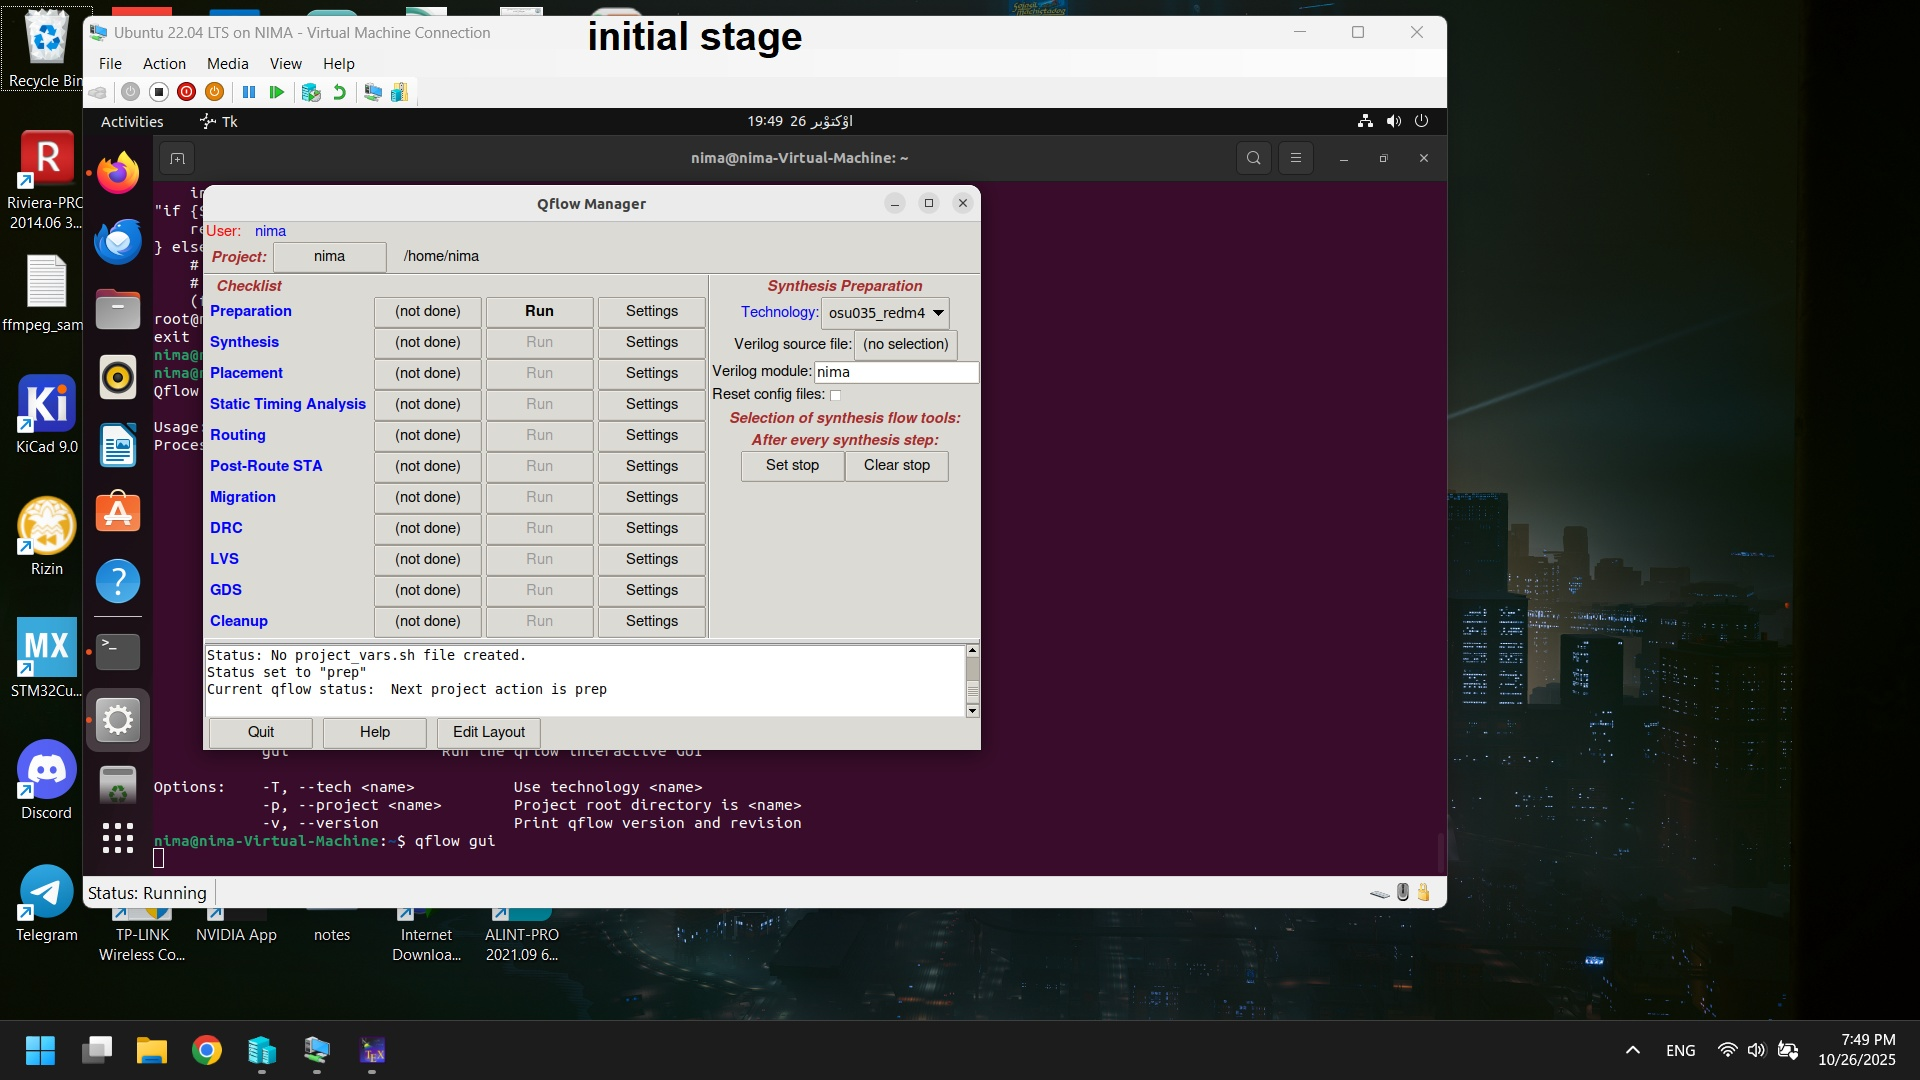
\includegraphics[scale=0.2]{init.jpg}
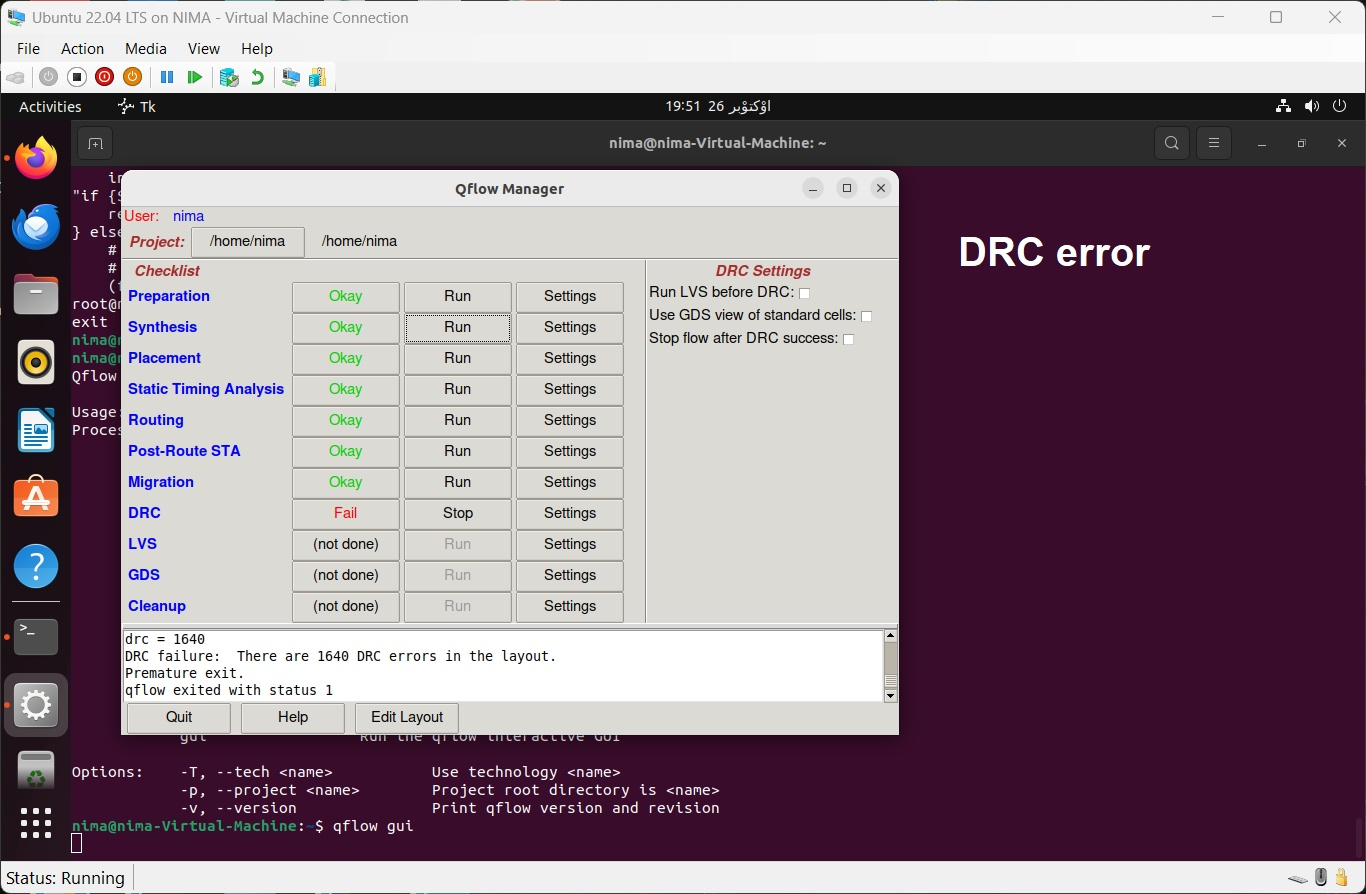
\includegraphics[scale=0.2]{drc.jpg}
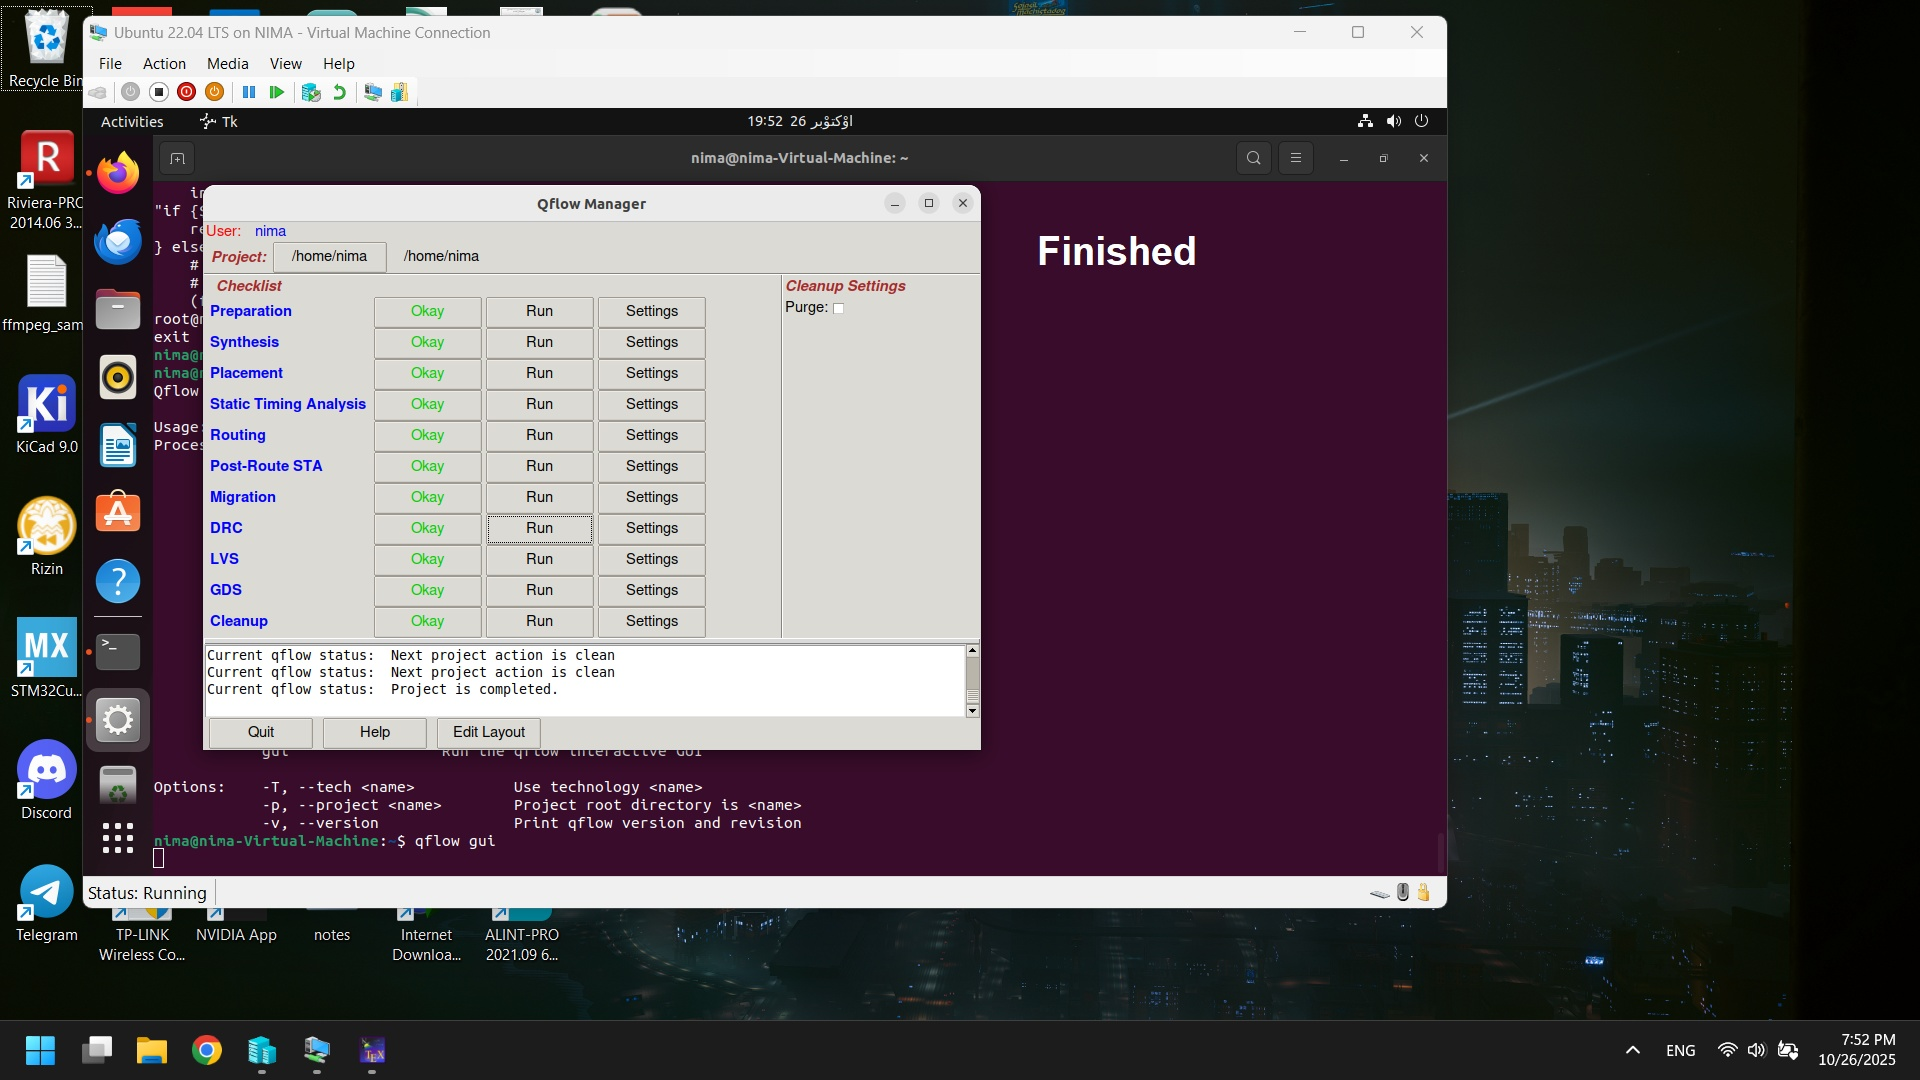
\includegraphics[scale=0.2]{finished.jpeg}
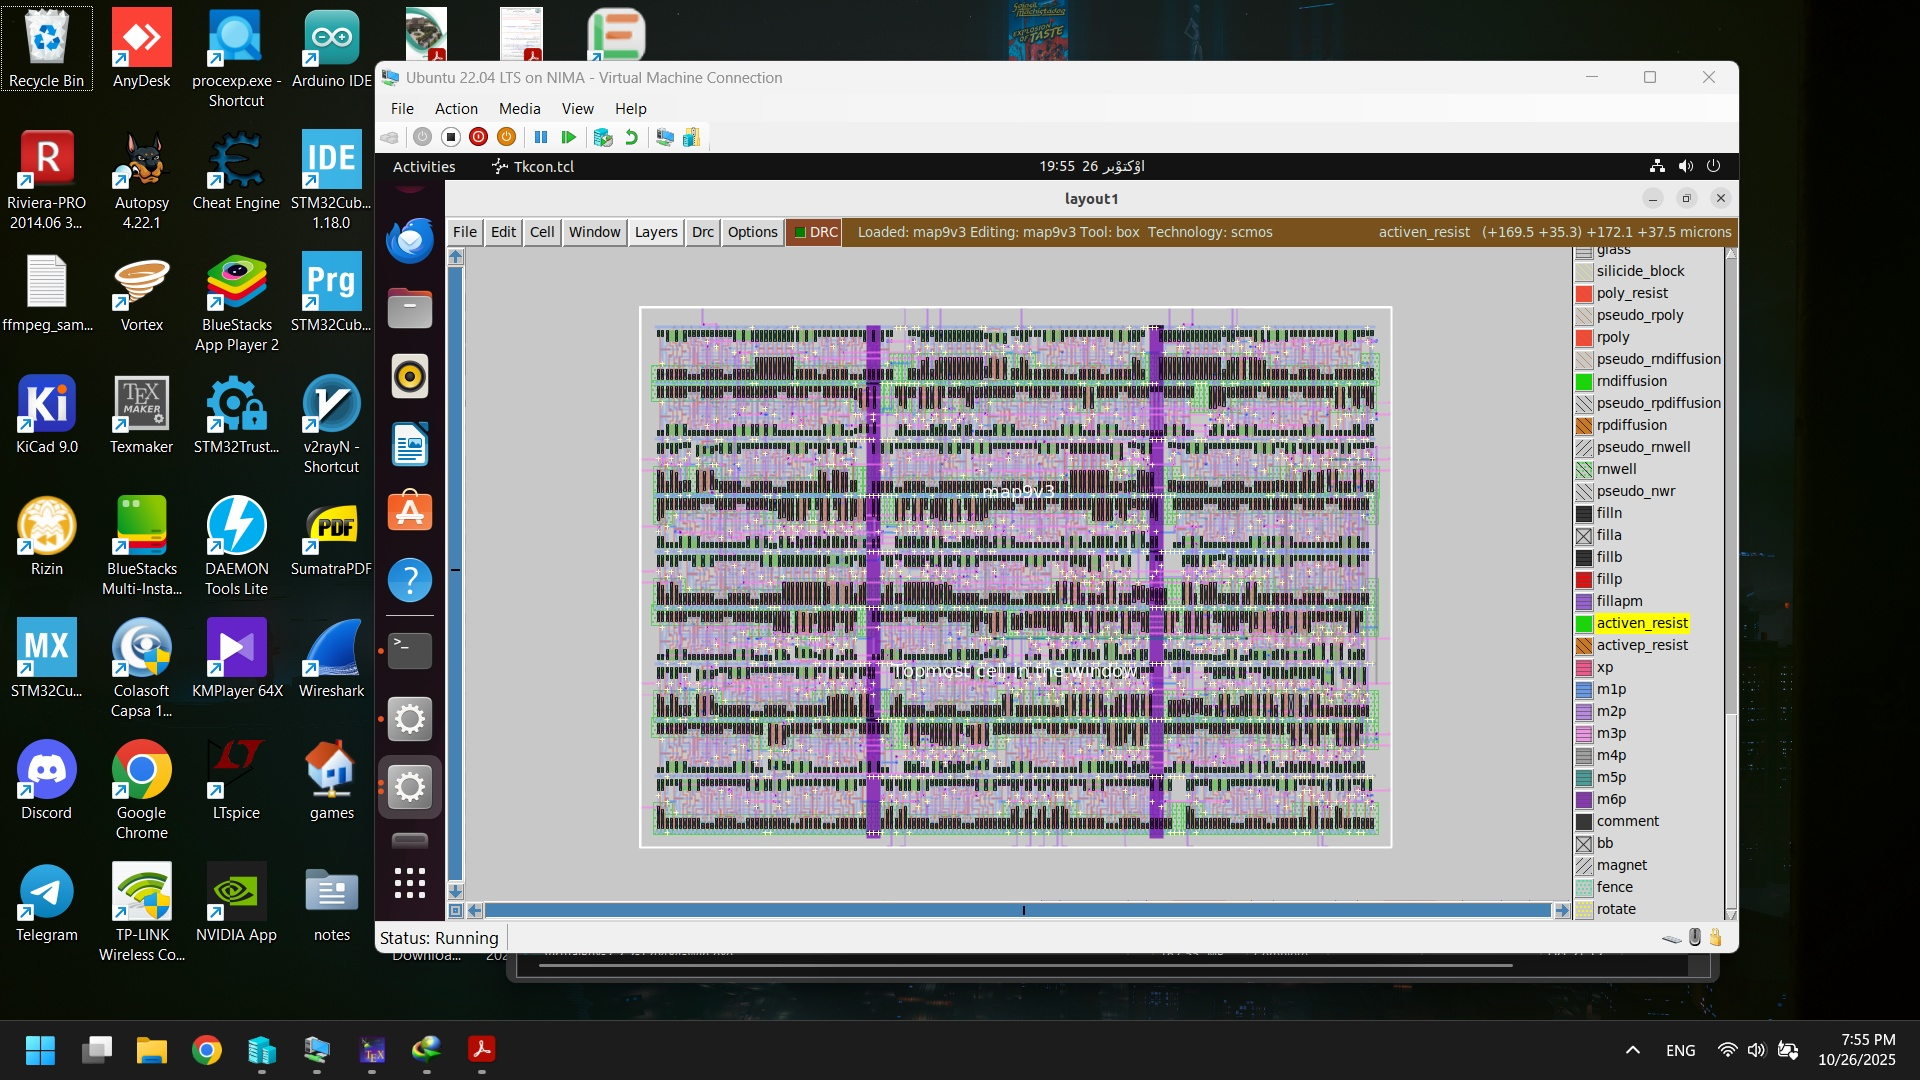
\includegraphics[scale=0.2]{layout.jpg}
\caption{QFLOW}
\end{figure}




\end{questions}


\end{document}